\chapter{Memory Management}

Memory management is import when compiling a program to be run in a resource
constrained environment. It is a topic of great interest in program compilation
in general. The problem is however simpler in the case of irreversible
languages. Once it is determined that some data is no longer needed it can
simply be deleted and reallocated as needed.

In a reversible computation memory management is somewhat complicated by the
reversibility constraint since a bit cannot be simply set to zero and reused
when it is no longer needed.

Thankfully since we are working in the circuit model determining if data is
needed in the future is simple (and computable!).

\section{Overview of Existing Approaches}

\subsection{Janus}
Janus\cite{YG:2007,LD:1982} is a reversible programming
language.  It's main focus is not to be a circuit description language, but to
be logically reversible. As a result of logical reversibility it does however have some
useful properties which help when compiling to circuits.

Janus guarantees that all programs implemented in it are reversible.
This reversibility is implemented at the statement level, that is to say that
all statements are reversible but the internals of a statement may not be.
This means that temporary ancilla may be allocated to compute a statement but
this ancilla can be cleaned up between statements.

\paragraph{Modification operators} are used for operations that can be done
in-place. For example the addition modification operator, \verb|+=|. Operations
that cannot be done in place can only occur to the right of an in place
operator. These operations can then be implemented, the result can be applied in
place to the left hand side value, and then cleaned up using Bennett if
necessary. This means that memory need only be allocated temporarily for each
modification statement.

\paragraph{If conditions} require a pre-condition (used to choose which branch
to take), and a post-condition (true if and only if the top branch is taken).
These are very useful in the context of memory management. The pre-condition can
be used to set a bit which controls which operations are preformed. The
post-condition can be used to clear this bit as the pre-condition may no longer
be true after the loop is preformed.

\todo{add diagram}

\subsection{Pebble Games and Garbage Collection}

Any computation where where execution is independent of input can be modeled as
a DAG. The nodes on the graph represent values and the arrow represent data
dependencies required for the computation of those values.

The \emph{Black Pebble Game} is a game played a DAG which is used to model
irreversible memory. The rules are as follows:
\begin{enumerate}
  \item A pebble can be added to a node if and only if all predecessors of the
    node have pebbles.
  \item A pebble can be removed at any time.
\end{enumerate}

Pebble games are often used to study space-time trade-offs in computing. For
example if we take some computation and model it as a DAG we can try and find
the minimum number of pebbles needed to compute some value in the graph. This
minimum corresponds to the minimal space cost of that computation.

\subsubsection{Reversible Pebble Game}

Bennett\cite{Bennett:89} describes an alternative pebble game for reversible
computation. The rules are similar to those used in the \emph{black pebble
game} except that the reversibility constraint prevents us from simply removing
pebbles. Each computation has a corresponding reverse computation, and the
dependencies of the reverse computation are the same as forward computation.
This means that pebbles may sill be removed but removal is subject to the same
conditions as placement. The rules for this version of the game are given below:

\begin{enumerate}

  \item A pebble can be added to a node if and only if all predecessors of the
    node have pebbles

  \item A pebble can be removed from a node if and only if all predecessors of
    the node have pebbles

\end{enumerate}

The space complexity of the game is given by the maximum number of pebbles which
are in play at any given time. It has been shown that in general computing the
space complexity for an arbitrary DAG is PSPACE-complete \cite{chan13}.

Strategies for playing these games have been analyzed in the case of, one
dimensional directed graphs, as well as for trees\cite{peb16}, for example

There are three particular strategies of interest in the 1D case:

The first is the naive strategy (sometimes called \emph{Bennett Method}). In
this strategy pebbles are added one after another until the desired pebble is reached.
All of the extra pebbles used in the computation are then removed in reverse
order. This strategy has time complexity $2n-1$ and space complexity
$n$.  This is the minimal time strategy in the 1D graph.

The second is a slightly more advanced strategy which will be referred to as the
\emph{incremental strategy}. Here we start with some limited number of pebbles
and place pebbles until we run out. After running out we uncompute all but the
last pebble following the Bennett strategy. This is then repeated using the next
pebble as the new starting point until the desired pebble is reached. This
strategy has a time complexity of $4n$ and a space complexity of
$\frac{1}{2}n^2$. Although this strategy is not optimal in all cases it is easy
to implement due to not requiring that the cleanup algorithm have prior
knowledge about the size of the circuit.

Finally the third is the optimal strategy (for a given space bound) from Knill \cite{knill:95}.
\todo{Briefly explain}

\section{MDD}

Lacking in the original pebble game is an effective way to represent mutation.
This is of not much consequence in the irreversible pebble game since mutation
can be modeled as a placement followed by the removal of a dependency. In the
reversible pebble game it is significantly more important since pebbles can
normally only be removed predecessors are pebbled.

For example addition via the mapping $(a,b) \mapsto (a,a+b)$ is a reversible
operation which does not require new space to be allocated for the result $a+b$.
In order for strategies from the reversible pebble game to be applied to a
circuit using this operation generically it would have to be made out of place
by copying the $b$ input and thus losing the advantages that may have been
gained by using an in-place operation.

In order to better represent in-place operations a new pebble game is proposed.
Rules one and two are similar to the reversible pebble game. The third rule
(as well as two types of labeled edges) has been added:

\begin{enumerate}

   \item A new pebble can be added to a node if and only if all predecessors of
     the node have pebbles.

   \item A pebble can be removed from a node if and only if all predecessors of
     the node have pebbles.

   \item A pebble may be moved forward or backward along a mutation edge if all
     predecessors of the destination node have pebbles.

\end{enumerate}

Note that since using the move described in the third rule is optional this is a
generalization of the reversible pebble game and any strategy that can be used
in the reversible pebble game is a valid strategy here. We also inherit the
PSPACE-completeness (\cite{chan13}) of solving the reversible pebble game since
any graph which does not include mutation edges is played by the rules of the
reversible pebble game.

As a simple example of the usefulness of such a game consider the computation of
$a+b+c$. In \cref{fig:mddExample} the reversible pebble graph as well as the MDD
are given. If the inputs ($a$,$b$,$c$) are considered to be pebbled then two
additional stones to pebble $a+b+c$ in the reversible pebble game. The first is
placed on $a+b$ and the second can then be placed on $a+b+c$. The MDD game on
the other hand needs only a single additional stone. In this case the stone will
be placed will to be placed on $a+b$ then slid along the modification path to
$a+b+c$.

\begin{figure}
  %\includegraphics[width=\textwidth]{images/pebExamples.tikz}
  \centering
  \begin{subfigure}{0.3\textwidth}
    \includegraphics{images/revPeb.tikz}
    \caption{Reversible}
  \end{subfigure}
  \qquad\qquad
  \begin{subfigure}{0.3\textwidth}
    \includegraphics{images/mddPeb.tikz}
    \caption{MDD}
  \end{subfigure}
  \label{fig:mddExample}
  \caption{The reversible pebble game and MDD for $a+b+c$}
\end{figure}


\subsection{Converting a Computation to an MDD}

First I will define the elements of the graph in terms of what they represent
with respect to computation:

\paragraph{Nodes} represent a register in some state.

\paragraph{Mutation Edges} represent operations which transform the value
of a register. The parent and child node of an edge represent the state of the
register before and after (respectively) the computation. Each node may have
only a single input and output mutation edge. A chain of nodes connected by
mutation edges represents all computations which change the contents of a
register.

\paragraph{Dependency Edges} point from values upon which a computation
depends. In order for a computation defined by a mutation edge to be implemented
all parent nodes along dependency edges pointing to the child node of the
mutation edge must be available.

For example the computation $(a,b)\mapsto(a,a+b)$ might be represented as a
solid arrow from the node $b$ to the node $a+b$ with a dependency arrow coming
from $a$.


\begin{theorem}
  For all MDDs a strategy to compute any particular value exists.
\end{theorem}

\begin{proof}

  Consider the following simple strategy.  First perform a topological sort of
  the node of the graph.  Now place a pebble on each node in the sorted order.
  It is guaranteed that the dependencies of each node will be pebbled since they
  are placed in sorted order. The entire graph may be covered by pebbles in this
  fashion.

\end{proof}

\todo{Other things that may be nice to prove, the construction of an MDD from a
      simple language show that the MDD computes the same function as the language.}


\subsection{Computing the Cost of a Strategy}

In order to compute the cost of a given strategy when it is applied a few
new rules are needed:

\begin{enumerate}
    \setcounter{enumi}{3}
  \item Each node has a computation cost which is payed when placing a new pebble on
    it or sliding an existing pebble to it.
  \item Each node has a space cost which gives the contribution of that node to
    the overall space complexity when it is pebbled.
  \item If a node has no parent it computes a constant so a pebble may be placed
    at any time.
\end{enumerate}

A implementation of a computation can be represented by an MDD and a list of
moves $\{m_i:i \in 1 \dotsc n\}$ (where $n$ is the total number of moves making up the
computation) where each move consists of a graph location and a move type. Given
a function $C$ which returns the gate cost of a move the total gate cost of a
computation is then:
\[ \sum_{i\in 1 \dotsc n} C(m_i) \]

Another way to represent the computation a set of states representing the graph
after each move $\{g_i:i \in 1 \dotsc n\}$. Given a function $S$ when returns
the total space in use for a state (by summing over the cost of all currently
placed pebbles) we can compute the space complexly as:

\[ \max_{i\in 1 \dotsc n} C(g_i) \]

The goal of this game is to come up with a set of moves the minimizes the total
movement cost as well as the space complexity.

When implementing the graph as a circuit we may preform the computations in any
valid topological ordering. Further if there are multiple computations which
could be next in a given ordering they can be preformed in parallel.

\subsection{Eager Cleanup}

If a value is no longer needed in a computation it can then be checked that the
information needed to clean it up is \emph{available}.  More precisely
\emph{available} is defined to mean that all dependencies needed to move the
pebble to the beginning of it's modification path currently have pebbles or have
pebbles that can be moved into place without causing additional space to be
used. If this is the case it can immediately be cleaned and the ancilla can be freed for
future use in the computation.

Eager cleanup is possible when all dependencies are \emph{one-way}.
This means that once there is no path from it to any of the modification paths
of it's dependencies (as shown in \cref{fig:one-way}).

\begin{figure}
  \centering
  \begin{subfigure}[b]{0.3\textwidth}
    \includegraphics[width=0.8\textwidth]{images/oneway.pdf}
    \caption{One Way}
    \label{fig:one-way}
  \end{subfigure}
  \qquad
  \begin{subfigure}[b]{0.3\textwidth}
    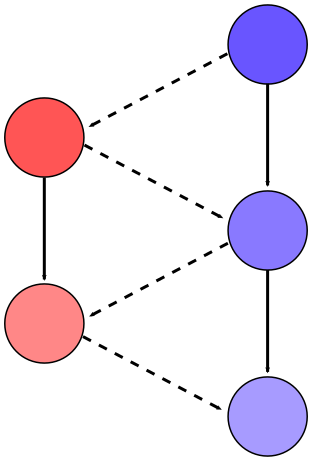
\includegraphics[width=0.8\textwidth]{images/interdependent.pdf}
    \caption{Interdependent}
    \label{fig:interdep}
  \end{subfigure}
\end{figure}

\todo{Write algorithm out formally and adapt the below proof sketch to the neewversion}

\begin{theorem}

Eager cleanup is possible on any graph with only one-way dependencies.  Let
$G=(V,E)$ be an MDD.  Assume that all mutation paths in $G$ are one-way
dependent\todo{define this}.\textsc{Eager} cleanup method in Algorithm
\ref{alg:eager} is correct in the sense that it all ancillas that may be used by
${\mathcal C}$ are returned in their initial state at the end of the
computation.

\end{theorem}

\begin{proof}
  \todo{This proof might be better with a diagram}
Our proof is by induction on the number $k$ of mutation paths $P_1, \ldots, P_k$
inside the MDD $G$. For the base $k=1$ there is only one mutation path, this
path either leads to an output, in which case no cleanup is necessary, or leads
to a node that has to be cleaned up. However, since all inputs to the path are
still available by assumption, the output of the path, i.e., its last node, can
simply be moved backward step by step, uncomputing each intermediate result,
until the initial state is recovered.

We strengthen the above statement by assuming that we can return the final state
of each path $P_1, \ldots, P_k$ to an arbitrary intermediate state.  Now, we
make the inductive step to $k+1$ paths. Recall that a node $v$ can be reversed
if all their dependency edges pointing to $v$ point from available nodes. (nodes
which are computable from the available data, by sliding a pebble up or down the
mutation path\todo{formalize this definition?}). We therefore make the inductive
step as follows: Assume that the paths $P_1, \ldots, P_{k+1}$ are arranged in
topological order. Let the $v$ be the node holding the current state of the last
path $P_{k+1}$, i.e., by assumption on the one-wayness of the graph, all edges
point into $P_{k+1}$ and none points backward. Now, consider all nodes in $P_1,
\ldots, P_k$ that would have to be available in order to move $v$ one step
backward. By induction, starting with $P_k$, we can slide the states for each
path into the location that is needed to make this information available for $v$
to move backward one step. Repeating this argument, we see that we can move the
state anywhere along the last path $P_{k+1}$ thereby showing that cleanup is
possible and algorithm \textsc{Eager} will find this cleanup strategy.

\end{proof}

\subsection{Triangles and Incremental Cleanup}

\Cref{fig:interdep} shows a graph where eager cleanup fails. The red mutation
path depends on previous values of the blue path in order to be cleaned.

It is still possible to clean up the blue node. A method for doing this is
somewhat related to the \emph{incremental strategy} discussed above generalized
to a DAG.

\subsection{Circuit Generation}
Circuit generation is defined by creating a generation function for each
type of move allowed in the game then using that set of functions to convert a
graph and move set into a circuit.

We start with a circuit consisting of registers corresponding to the input nodes
of the graph.

A heap of currently available ancilla is kept. This ensures that the
lowest available numbered ancilla is always the one allocated so ancilla use is
minimized.

\begin{itemize}
    \item Place Pebble: Place circuit which computes the function at the node
      using the nodes dependencies as input. Assign ancilla for the output of
      the circuit from the heap.
    \item Remove Pebble: Place the reverse circuit for the function at the node
      using dependencies as input, uncomputing the previously computed value.
      Return previously assigned ancilla to the heap.
    \item Slide Pebble: Place circuit which computes the function at the node
      using the nodes dependencies as input and the bits representing the
      current value of the node as the modified input.
\end{itemize}

\todo{prove, under some assumptions, that this procedure constructs a circuit
        computing the same function as the MDD }

\subsection{Example: SHA-256}

Larger scale example of compilation with MDD can be see in SHA.
\todo{The main goal in this example is to show that SHA can be automatically
  compiled to use no additional ancilla per round. This can also be done using
  the Janus modification operator scheme on it's own so it may nice to show
another example where that fails.}

\begin{figure}[ht]
      \capstart
      \centering
      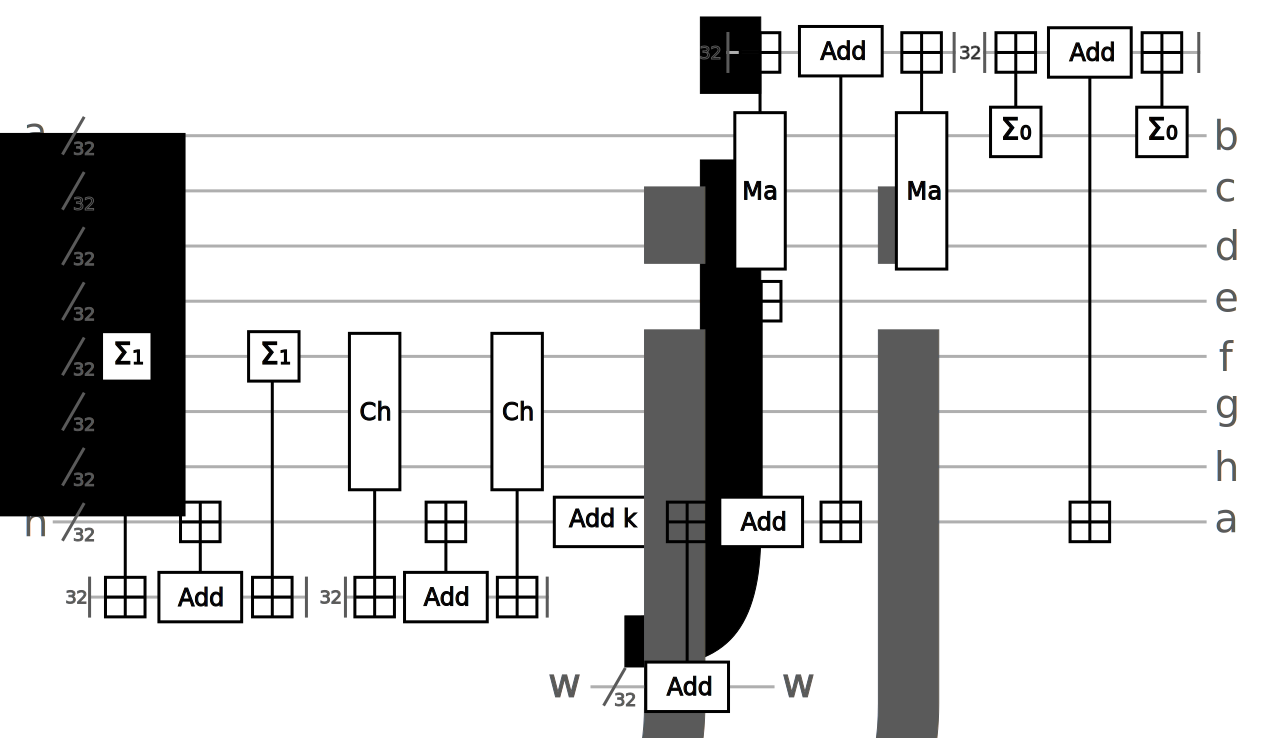
\includegraphics[width=0.9\hsize]{images/sha_round}
      \caption{One Round of SHA-256}
      \label{fig:sha}
\end{figure}

